
\chapter{MODELLING OF WEB APPLICATIONS VIA STATE MACHINE}

\section{Generation of State Machine Model}

 State Machine for a Web Applications is characterized with a three tuple (r, V, E)
 \begin{itemize}
     \item V is the list of vertices which is recognized as the DOM States in the model
     \item E is the edges or transitions associated with States after clicking capable events(candidate elements).
     \item r is the root element or initial State of the model 
 \end{itemize}
 
Crawljax, a open source tool is used to generate the State machine model for web applications. It uses selenium webdriver as a event handler to make direct calls to the browser. The url of web application is the input to create State machine. The browser is intialized and the DOM tree of the web application is extracted and the DOM State is created as the root element. The next step is to find the clickable events in the webpage, both static elements(HTML hyperlinks) and javascript events(eg. Onclick events). These elements are determined as candidate elements for firing transitions in the webpage. Candidate elements are activated one by one and the resulting DOM tree is extracted. The resulting DOM tree is compared with the existing DOM States by the use of a comparator. The DOM tree is converted into strings and the string is the matched with the result State is added to the State machine with an edge added to the previous State. The candidate element from which the transition is done is now removed from the list and the previous State is restored. All the States reachable from the initial State is determined by firing events with all candidate events. This crawl procedure is done for a maximum crawl depth as defined initially.\\
\newline
The below figure illustrates a example web application and its corresponding State machine model.

\section{Example of a Web Application and its Model}

The below figure represents the web application http://www.testfire.net/

\begin{figure}[!h]
 \begin{center}
    \resizebox{100mm}{75mm} {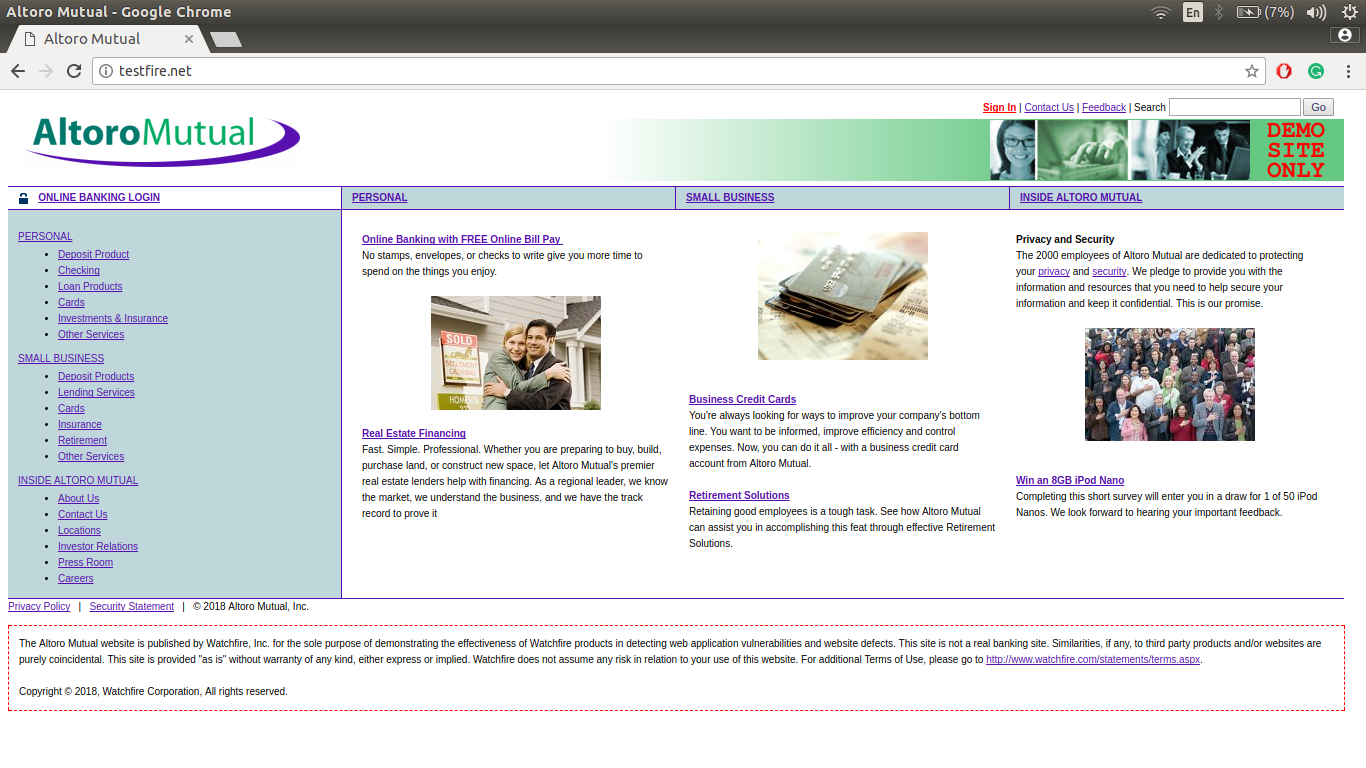
\includegraphics {Chapters/Testfire.eps}}
    \caption {A example banking web application}
  \label{fig:Table}
 \end{center}
\end{figure}

\subsection{Crawl Level 1}

The below figure is a state machine model for web application http://www.testfire.net/ with crawl level 1. In crawl level1, initial start DOM state is home page of web applications and all the state reachable from the start state is modelled.

\begin{figure}[!h]
 \begin{center}
    \resizebox{100mm}{75mm} {\includegraphics {Chapters/Crawl1.eps}}
    \caption {State Machine Model for Crawl Level 1}
  \label{fig:Table}
 \end{center}
\end{figure}

\subsection{Transition between states}
Let us consider the transition between states- start state(index page) to state 39.
\\
$ "from" : "index",
  "to" : "state39" $
  \\

The transition is caused the event type click  through the element submit button having value Go. \\
$
  "element" : "Element{node=[INPUT: null], tag=INPUT, $ \\ $text=, attributes={type=submit, value=Go}}",
  "eventType" : "click" $
\\

The submit button is present in the DOM tree path as show below. \\
$ 
  "id" : "xpath /HTML[1]/BODY[1]/DIV[1]/FORM[1]/TABLE[1]/TBODY[1]/$\\ $TR[1]/TD[2]/INPUT[2]",
 $\\
 
Similarly, the transition between the states- (index page) to state35 can be explained as below.
$
{
  "from" : "index",
  "to" : "state35",
 $\\
 
 The transition is caused by selecting a hyperlink default.aspx?content=security.htm
 $
  "element" : "Element{node=[A: null], tag=A, text=security, $ \\ $attributes={href=default.aspx?content=security.htm}}",
  "eventType" : "click"
}$
\\

The hyperlink is present in the DOM tree path below\\
$
 "id" : "xpath /HTML[1]/BODY[1]/DIV[2]/TABLE[1]/TBODY[1]/$ \\$ TR[2]/TD[2]/SPAN[1]/TABLE[1]/TBODY[1]/TR[1]/TD[3]/A[2]",
 $


\subsection{Crawl Level 2}

 In crawl level 2, the states reachable from start state are captured and the modelling procedure is repeated with these states as starting states unlike crawl level 2. The below figure is a State Machine Model derived from web applications http://www.testfire.net for a crawling level of 2.

\begin{figure}[htpb]
 \begin{center}
    \resizebox{150mm}{125mm} {\includegraphics {Chapters/Crawl2.eps}}
    \caption {State Machine Model for Crawl Level 2}
  \label{fig:Table}
 \end{center}
\end{figure}
